\documentclass[12pt]{article}

\usepackage{amssymb,amsmath,amsthm}
\usepackage{graphicx}
\usepackage{pgfplotstable,booktabs,longtable}
\usepackage{float} % Package for including figures
%\usepackage{psfrag,color}

\title{Homework 6 \protect \\(Math/CS 471)}

\author{Elijah Perez \protect \newline \\ Natalie Chang}


\date{\vfill 11/24/2020}   



\begin{document}
	\maketitle
	\pagebreak
	
	\section{Introduction}
    In this report we will explore the efficiency benefits of parallel computing compared to serial computing. Specifically, we will look at Open Multi-Processing. We will do this by calculating partial derivatives using finite difference methods as well as the error of these derivatives using a two dimensional integral that is calculated using a two dimensional trapezoid rule. We will also test the scalability of the program using both weak scaling and strong scaling. Tests will be conducted on Stampede 2, the 21st fastest supercomputer in the world as of June 2020. The goal of this report is to show the speed up and efficiency of using parallel programming, as well as evaluating the accuracy of the derivatives and integral calculations. The method used can be found in the Method section, the results can be found in the Results section, and any final remarks and notes of improvement can be found in the Conclusion section.
	
	\section{Method}
	The function that is being differentiated is:
	\begin{equation}
		u(x,y)=sin(x)cos(x), \hspace{2mm} x(r,s)=r+0.1s,\hspace{2mm} y(r,s)=s
	\end{equation}
	Where $(x,y)\in \Omega$, and $(r,s)\in \Omega_R=[-1,1]^2$
	\newline
	\newline
	The partial derivatives, $u_x(x,y)$ and $u_y(x,y)$ are approximated using finite difference methods. The error of the approximate derivatives to the true derivatives is found by the following integral:
	\newline
	\begin{equation}
		e_2(h)=(\ \int_\Omega \![u_x(x,y)+u_y(x,y)-u_{x,exact}(x,y)-u_{y,exact}(x,y)]^2dxdy\ )\ ^{0.5}
	\end{equation}
	This integral in (2) is calculated using a two dimensional trapezoid rule.
	\newline \newline
		To show the benefits of parallel computing in this report, two tests were conducted. These will also test the scalability of our program. Scalability refers to the ability of a parallel system (software and/or hardware) to demonstrate a proportional increase in parallel speedup with the addition of more resources.
		 In the first test, we had strong scaling, where the grid size is independent of the number of threads with grid sizes $20 \times 20$ and $800 \times 800$. The goal is to run the same problem size faster. Perfect scaling means that the problem is solved in $\frac{1}{n_p}$ time, compared to serial computation where $n_p$ is the number of processors. The second test explores weak scaling, where the grid size is proportional to the thread count with grid sizes $200 \sqrt{n} \times 200 \sqrt{n}$ where $n$ is the number of threads ranging from 1 to 16, and the grid size is rounded to the closest integer. The goal is to run a larger problem in the same amount of time. For this experiment we are using the Stampede 2 supercomputer with 4200 Dell KNL compute nodes, each including 68 cores. For maximum efficiency it is recommended to only use one thread per core. Therefore, throughout this report the thread count and core count are interchangeable. 
	\newline\newline
	To make this code parallel, we used OpenMP (Open Multi-Processing) for Fortran. OpenMP works by dividing tasks between threads, so that tasks can be completed simultaneously. A fork-join model best represents this concept. If only one thread is called for the OpenMP program, then it is running as a serial program. This one thread is the master thread. Every OpenMP program has a master thread. When the program reaches a parallel section, the master thread calls a team of threads to compute the next tasks, depending on the options decided by the programmer. A sucessful OpenMP program can be compiled with and without OpenMP flags and still produce the same results. For maximum efficiency, we have implemented OpenMP to the main program and any modules/subroutines that it uses. 
\newline \newline
The main constructs used include parallel blocks, looping, single blocks, and barriers. Since our code involved large grid sizes, using 'omp do' (OpenMP's parallel do loop construct) loops to create the grid matrices was effective in decreasing the run time. With a large grid size, there are many tasks to divide between threads. Specifically, using a static schedule was more efficient than dynamic. This could be explained by an increase in parallel overhead. Parallel overhead is the amount of time required to coordinate parallel tasks, as opposed to doing useful work. The dynamic scheduling type has higher overhead than the static scheduling type because it dynamically distributes the iterations during the runtime. Furthermore, nested loops utilized the collapse clause which makes both the outer and inner loop more efficient.  
	\newline \newline
	Another technique used to decrease the run time was strategic placement of the 'no wait' clause and implicit barriers. Implicit barriers were placed when the following code included variables that were dependent on earlier calculations. This is seen mainly in homework4.f90 in the early stages of the program where matrices are being initialized using loops. Where necessary, the single construct is used to avoid values being overwritten by other threads. These are critical calculations to the overall program. This could have also been achieved by using the 'critical' construct, however, this would have increased the parallel overhead time which is something that we want to avoid. In homework4.f90, line 149 uses a reduction clause which is another way to protect critical calculations without significantly impacting efficiency. These are all techniques used to ensure that no new error is incurred by the parallel code.   
\newline \newline
	To calculate the results, the runtime of the program was found by taking the average time over 10 repetitions using the built in 'omp\_get\_wtime' function. The speed up was calculated by finding the difference between the runtime at thread count $x$ and the runtime at thread count 1. These metrics were imported into MATLAB and used to create the plots shown in the Results section.

	\section{Results}
	First, we will show that no new error was introduced from the parallel code. Since the partial derivatives were approximated using finite difference methods, we introduced some error in the calculation. This error was approximated using (2). 
 Figures 1 and 2 below show that running the program parallel or serial does not change the result of the error calculation, meaning that the implementation of parallel methods did not effect the results. This is one aspect of a successful OpenMP program.
	



	Figures 3 and 4 show the runtimes of the program at each thread count of the strong scaled problem. The overall trend is that as thread count increases, the runtime decreases. 

		\begin{figure}[H]
		\centering
		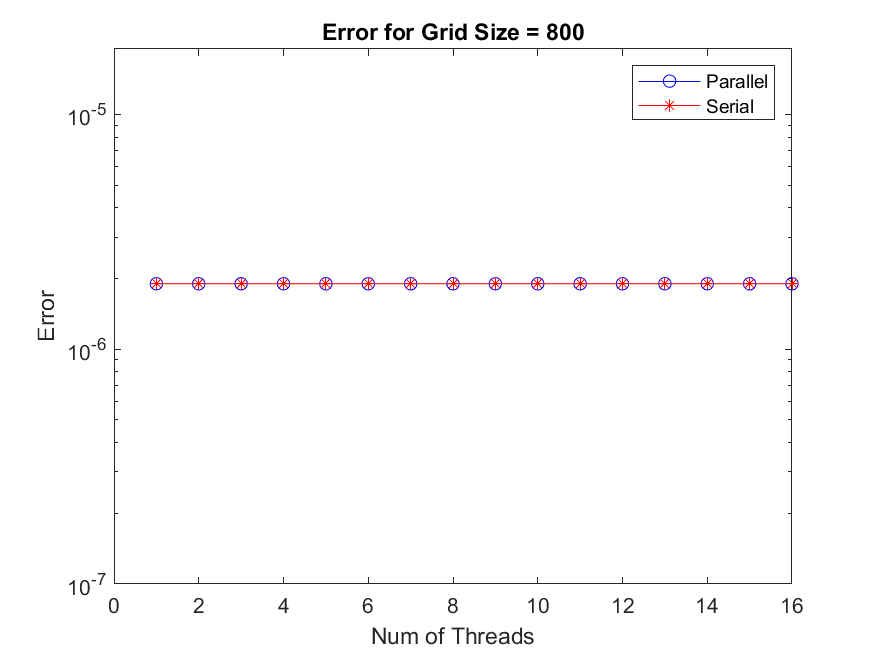
\includegraphics[width=100mm,height=80mm]{errorVthread800.png}
		\caption{Strong scaling: Error calculated using (2) for a grid size of $800\times800$}
	\end{figure}
	
	\begin{figure}[H]
		\centering
		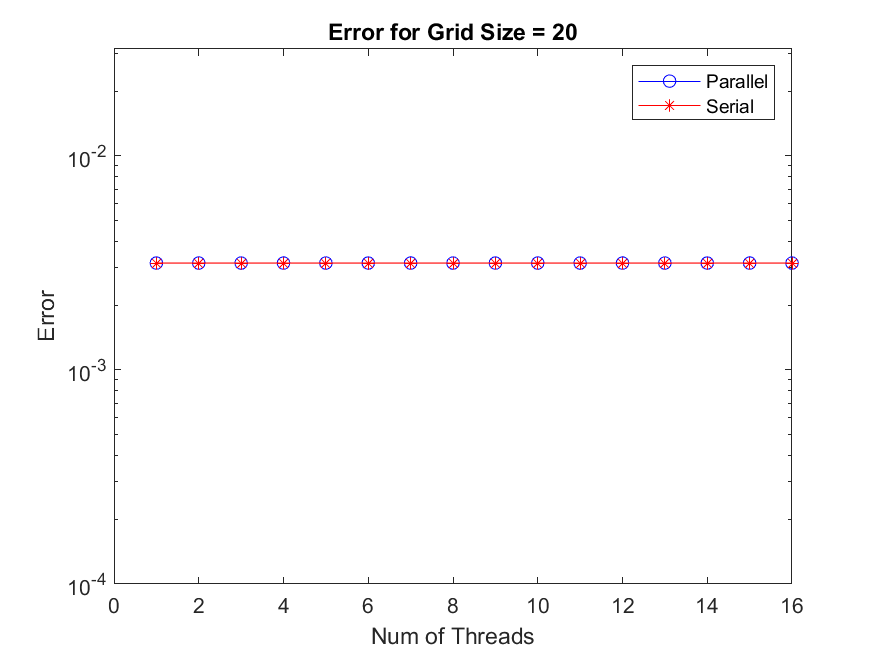
\includegraphics[width=100mm,height=80mm]{errorVthread20.png}
		\caption{Strong scaling: Error calculated using (2) for a grid size of $20\times20$}
	\end{figure}
	\begin{figure}[H]
		\centering
		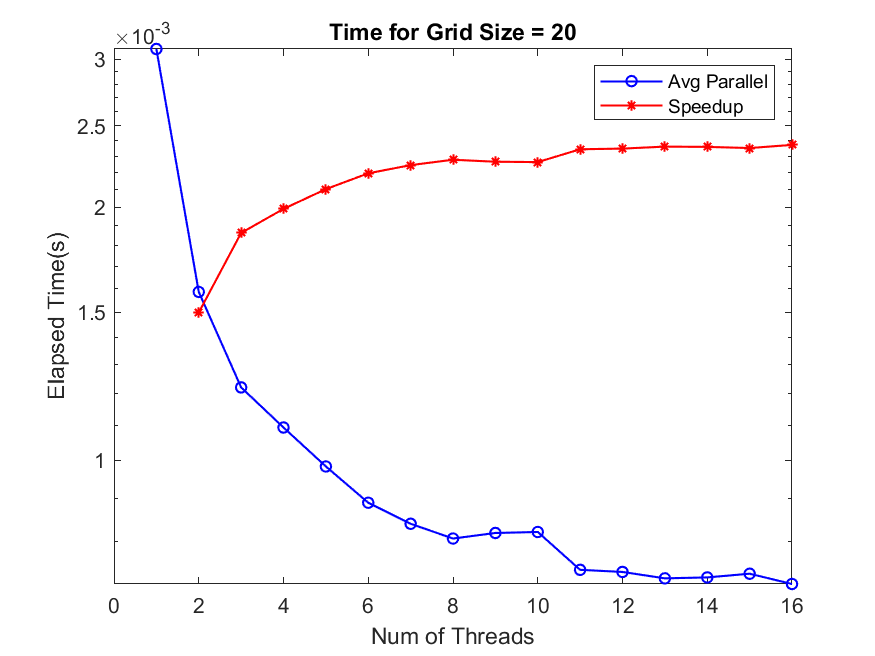
\includegraphics[width=100mm,height=80mm]{timeVthread20.png}
		\caption{Strong scaling: Runtime vs thread count on $20\times20$ grid}
	\end{figure}

	\begin{figure}[H]
	\centering
	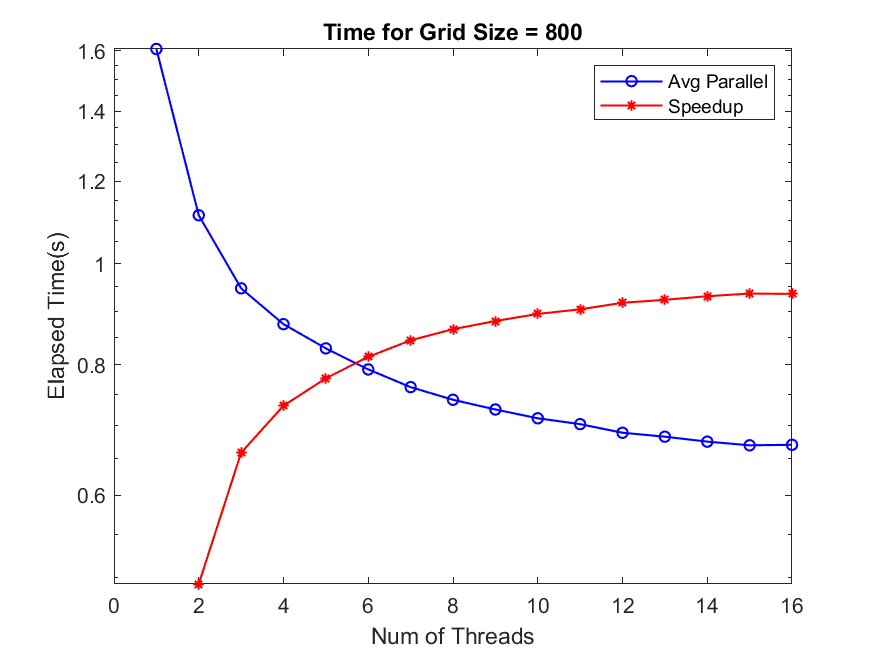
\includegraphics[width=100mm,height=80mm]{timeVthread800.png}
	\caption{Strong scaling: Runtime vs thread count on $800\times800$ grid}
\end{figure}
	\newpage
	Now, looking at the weak scaling we still see that no new error was incurred from making the code parallel. This can be seen in Figure 5. This also shows that the serial code converges as expected since an increase in grid size decreases the error found using (2). When comparing the runtime for parallel vs serial, the serial time had to be calculated individually at each grid size. This is why the plot in Figure 6 is represented differently than in the strong scaled problem. Figure 6 shows the runtime for the weak scaled problem. 

		\begin{figure}[H]
		\centering
		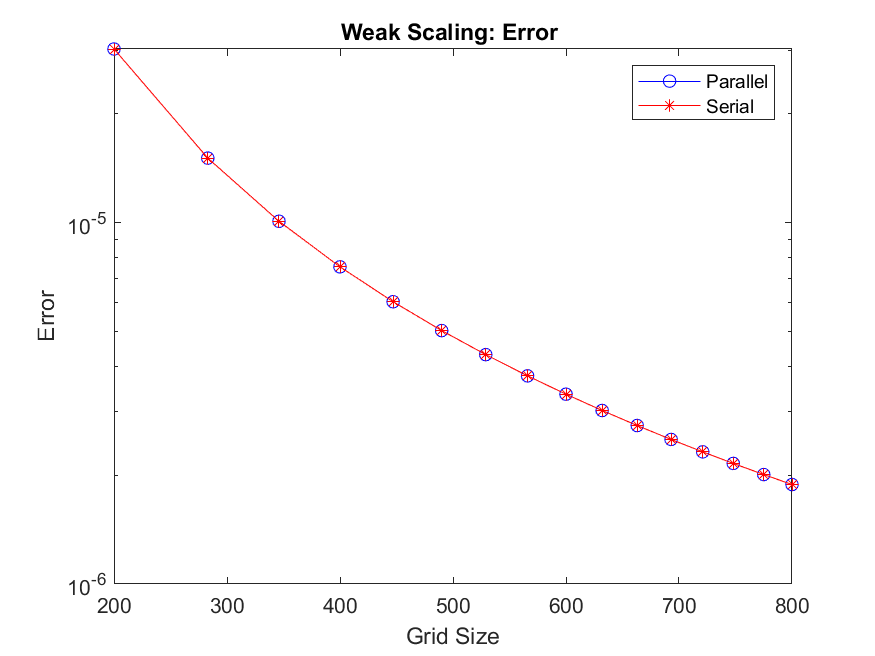
\includegraphics[width=100mm,height=80mm]{weakerror.png}
		\caption{Weak scaling: Error calculated using (2)}
	\end{figure}
	\begin{figure}[H]
		\centering
		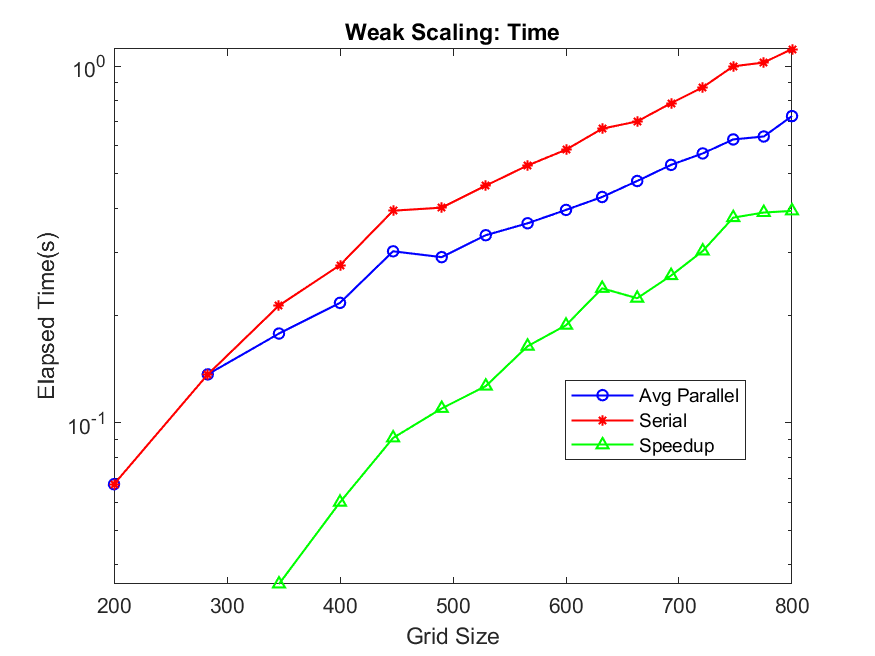
\includegraphics[width=100mm,height=80mm]{weaktime.png}
		\caption{Weak scaling: Serial vs Parallel Runtime}
	\end{figure}
		\newpage	
		%\begin{figure}
		%	\centering
		%	\includegraphics[width=100mm,height=60mm]{File here}
		%	\caption{Caption here}
		%\end{figure}
		%\vspace{1in}
		
		
        \section{Conclusion}
    	From the results we can conclude that the error (2) did not change when we made the code parallel. This is seen in Figures 1,2 and 5. The results are completely independent of the number of threads used.
    	\newline \newline
    	 For the strong scaled problem, we saw speed up with increased thread count. We can conclude that our problem is scalable with strong scaling and responds well to an increased thread count. This means that we can run the same problem size faster by using more threads. The flattening of the red speedup curves in Figures 3 and 4 demonstrate a diminishing return on speed up with increased thread count. It is possible that with a larger problem size, the diminishing return will be lessened since, with a larger problem size, there are more tasks to share between threads. This can be tested by further increasing the grid size.
    	\newline \newline
    	With weak scaling we wanted to see constant run time with increased grid size. We did not directly see this result, however we did see improvements in parallel run time over serial. One way to see better performance through weak scaling could be to use less grid points per core. For example, instead of having grid size $200\sqrt{n}\times200\sqrt{n}$ we could have $200n^{0.25}\times200n^{0.25}$, where n is the number of threads. Nonetheless, the larger problem was not computed in the same amount of time, hence our problem and program did not respond well to the weak scaling.
    	\newline \newline
    	One way to improve our parallel code would be to improve the efficiency of certain sections of the program. We found where the program was spending the most time by setting timers at different milestones in the code and analyzing the time spent between sections compared to that of the serial time. After doing this we can conclude that lines 122 through 134 and lines 139 through 143 could greater utilize OpenMP constructs. These sections of code are nested loops that use addition, subtraction, multiplication, and division. When we use the same constructs as the other nested loops in our program, it caused the runtime of these sections to increase with thread count. This is why these sections currently run under the single construct in our code. With greater knowledge of OpenMP and more testing, we could find a better way to utilize parallel programming for these sections. 

\end{document}  
